\documentclass[11pt,t,usepdftitle=false,aspectratio=169,usenames,dvipsnames]{beamer}
\usetheme[nototalframenumber,foot,logo]{uibk}
\headerimage{3}

\usepackage[T1]{fontenc}
\usepackage{xcolor}
\usepackage{minted}
\usepackage{tikz}
\usetikzlibrary{calc}

\definecolor{uibkBlue}{HTML}{00325c}
\definecolor{uibkOrange}{HTML}{ff9027}

\title{Reimplementing CoAP for C\# with the Task-based Asynchronous Pattern}
\subtitle{Is it worth to await?}
\author{Philip Wille}

\begin{document}
    \maketitle{}

    \begin{frame}
        \frametitle{Introduction}
        \begin{itemize}
            \item<1-> Synchronous and asynchronous execution
            \begin{itemize}
                \item<2-> Synchronous:
                \begin{itemize}
                    \item<3-> \textcolor{uibkBlue}{\textbf{Waiting for completion}} of method before continuing with program flow.
                    \item<5-> \textcolor{uibkBlue}{\textbf{Busy waiting}} $\rightarrow$ Thread is marked as \textcolor{uibkBlue}{\textbf{blocked}}.
                \end{itemize}
                \item<2-> Asynchronous:
                \begin{itemize}
                    \item<4-> Can \textcolor{uibkBlue}{\textbf{perform other tasks}} while the execution is running.
                    \item<6-> \textcolor{uibkBlue}{\textbf{No busy waiting}} $\rightarrow$ Thread is \textcolor{uibkBlue}{\textbf{free}} for other tasks.
                \end{itemize}
            \end{itemize}
            \item<7-> \textcolor{uibkBlue}{\textbf{T}}ask-based \textcolor{uibkBlue}{\textbf{A}}synchronous \textcolor{uibkBlue}{\textbf{P}}attern (TAP)
            \begin{itemize}
                \item<8-> Developed by Microsoft.
                \item<9-> Simple usage.
                \item<10-> Built-in in C\#.
            \end{itemize}
            \item<11-> \textcolor{uibkBlue}{\textbf{Co}}nstrained \textcolor{uibkBlue}{\textbf{A}}pplication \textcolor{uibkBlue}{\textbf{P}}rotocol (CoAP)
            \begin{itemize}
                \item<12-> Subset of \textcolor{uibkBlue}{\textbf{H}}yper\textcolor{uibkBlue}{\textbf{t}}ext \textcolor{uibkBlue}{\textbf{T}}ransport \textcolor{uibkBlue}{\textbf{P}}rotocol (HTTP).
                \item<13-> Specialized for \textcolor{uibkBlue}{\textbf{I}}nternet \textcolor{uibkBlue}{\textbf{o}}f \textcolor{uibkBlue}{\textbf{T}}hings (IoT) and \textcolor{uibkBlue}{\textbf{M}}achine-\textcolor{uibkBlue}{\textbf{t}}o-\textcolor{uibkBlue}{\textbf{M}}achine (M2M) devices.
            \end{itemize}
        \end{itemize}
    \end{frame}

    \begin{frame}
        \frametitle{Synchronous execution}
        \begin{figure}[ht]
            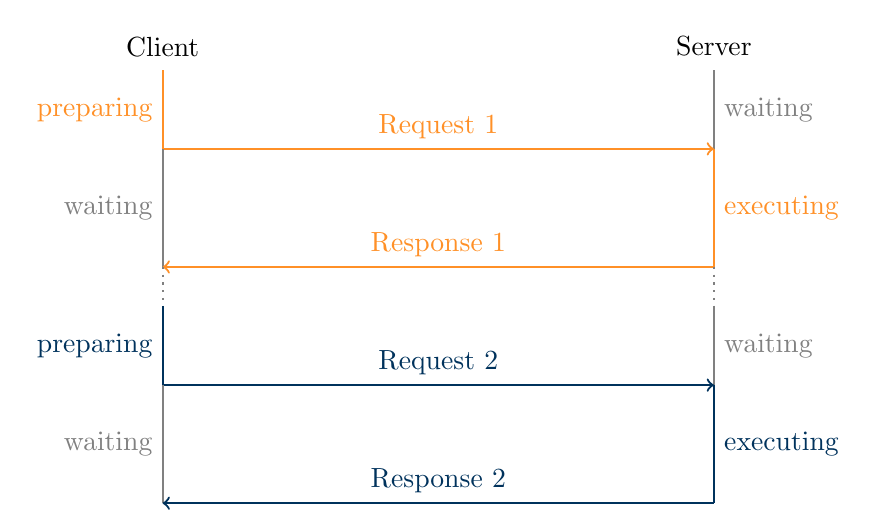
\begin{tikzpicture}
                \node at (-3,.3) {Client};
                \node at (4,.3) {Server};

                \draw[thick, uibkOrange] (-3,0) -- node[left] {preparing}(-3,-1);
                \draw[thick, gray] (4,0) -- node[right] {waiting} (4,-1);
                \onslide<1->
                \draw[->, thick, uibkOrange] (-3,-1) -- node[midway,above] {Request 1} (4,-1);
                \onslide<2->
                \draw[thick, gray] (-3,-1) -- node[left] {waiting} (-3,-2.5);
                \draw[thick, uibkOrange] (4,-1) -- node[right] {executing} (4,-2.5);
                \onslide<3->
                \draw[<-, thick, uibkOrange] (-3,-2.5) -- node[midway,above] {Response 1} (4,-2.5);
                \onslide<4->
                \draw[dotted, thick, gray] (-3, -2.5) -- (-3, -3);
                \draw[dotted, thick, gray] (4, -2.5) -- (4, -3);
                \onslide<5->
                \draw[thick, uibkBlue] (-3,-3) -- node[left] {preparing}(-3,-4);
                \draw[thick, gray] (4,-3) -- node[right] {waiting} (4,-4);
                \onslide<6->
                \draw[->, thick, uibkBlue] (-3,-4) -- node[midway,above] {Request 2} (4,-4);
                \onslide<7->
                \draw[thick, gray] (-3,-4) -- node[left] {waiting} (-3,-5.5);
                \draw[thick, uibkBlue] (4,-4) -- node[right] {executing} (4,-5.5);
                \onslide<8->                
                \draw[<-, thick, uibkBlue] (-3,-5.5) -- node[midway,above] {Response 2} (4,-5.5);
            \end{tikzpicture}
        \end{figure}
    \end{frame}

    \begin{frame}
        \frametitle{Asynchronous execution}
        \begin{figure}[ht]
            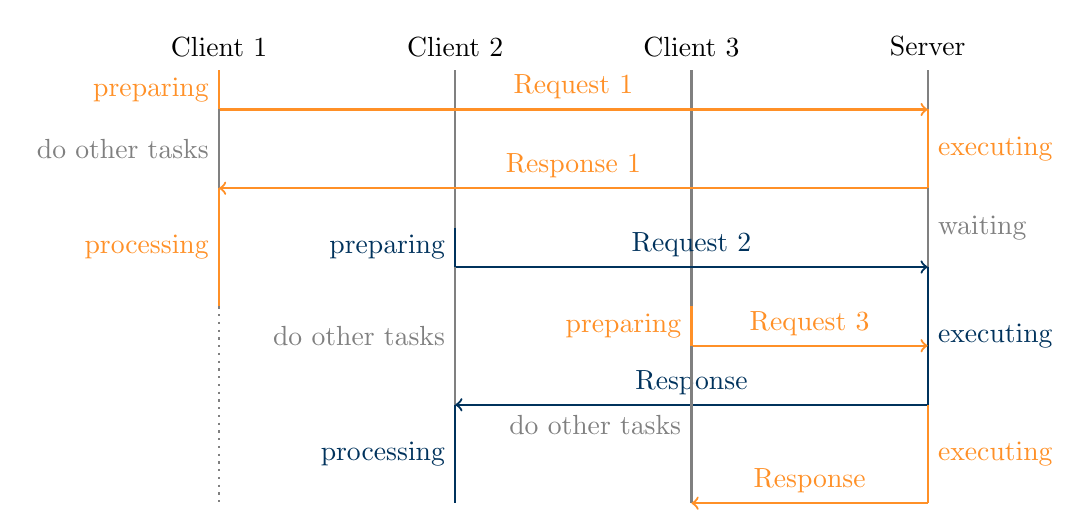
\begin{tikzpicture}
                \node at (-3,.3) {Client 3};
                \node at (-6,.3) {Client 2};
                \node at (-9,.3) {Client 1};
                \node at (0,.3) {Server};

                \draw[thick, uibkOrange] (-9,0) -- node[left] {preparing}(-9,-0.5);
                \draw[thick, gray] (-6,0) -- (-6,-2);
                \draw[thick, gray] (-3,0) -- (-3,-3);
                \draw[thick, gray] (-0,0) -- (0,-0.5);
                \onslide<1->
                \draw[->, thick, uibkOrange] (-9,-0.5) -- node[midway,above] {Request 1} (0,-0.5);
                \onslide<2->
                \draw[thick, gray] (-9,-0.5) -- node[midway, left] {do other tasks} (-9,-1.5);
                \draw[thick, uibkOrange] (0,-0.5) -- node[right] {executing} (0,-1.5);
                \onslide<3->
                \draw[<-, thick, uibkOrange] (-9,-1.5) -- node[midway, above] {Response 1} (0,-1.5);
                \onslide<4->
                \draw[thick, uibkOrange] (-9,-1.5) -- node[midway, left] {processing} (-9,-3);
                \draw[thick, gray] (0,-1.5) -- node[midway, right] {waiting} (0,-2.5);
                \draw[thick, uibkBlue] (-6,-2) -- node[left] {preparing} (-6,-2.5);
                \onslide<5->
                \draw[dotted, thick, gray] (-9,-3) -- (-9,-5.5);
                \draw[->, thick, uibkBlue] (-6,-2.5) -- node[midway, above] {Request 2} (0,-2.5);
                \onslide<6->
                \draw[thick, uibkOrange] (-3,-3) -- node[left] {preparing} (-3,-3.5);
                \onslide<7->
                \draw[thick, gray] (-6,-2.5) -- node[midway, left] {do other tasks} (-6,-4.25);
                \draw[thick, uibkBlue] (0,-2.5) -- node[midway, right] {executing} (0,-4.25);
                \draw[->, thick, uibkOrange] (-3,-3.5) -- node[midway, above] {Request 3} (0,-3.5);
                \onslide<8->
                \draw[<-, thick, uibkBlue] (-6,-4.25) -- node[midway, above] {Response} (0,-4.25);
                \onslide<9->
                \draw[thick, uibkBlue] (-6, -4.25) -- node[midway, left] {processing} (-6, -5.5);
                \draw[thick, uibkOrange] (0,-4.25) -- node[midway, right] {executing} (0,-5.5);
                \draw[thick, gray] (-3,-3.5) -- node[midway, left] {do other tasks} (-3,-5.5);
                \onslide<10->
                \draw[<-, thick, uibkOrange] (-3,-5.5) -- node[midway, above] {Response} (0,-5.5);
            \end{tikzpicture}
        \end{figure}
    \end{frame}
\end{document}